
%% %%
%% %% INTRO
%% %%

\slide{ A vs C side asymmetry: status }
{
\only<1> {
  Recall that we saw strong evidence that there is a \red{serious problem} with the \red{mu18MG triggers on the C-side}. These problems \red{cannot be corrected with Z tag-and-probe} because of the (yet unknown) bug with AOD and D3PD-based trigger matching. \\
A possible way out: switching over to mu18 triggers (or even using both: mu18-OR-mu18MG).
}
\only<2> {
  \red{Bad news}: Takashi Matsushita, the muon trigger and trigger SF expert, left ATLAS 3 days ago and cannot work on this anymore.
}
\only<3> {
  \red{Good news}: Carl Jeske, who worked with Takashi in the past, was able to take over. Today, I'll compare the results obtained with mu18-only trigger and Carl's new trigger SFs (labeled ``LATEST'') with mu18MG-only trigger and the default SFs (labeled ``BEFORE'').
}
}

% W ratios
\slide{ BEFORE: W ratio }
{
\colb[T]
\column{.5\textwidth}
\centering
\small{ $W^{+}$}
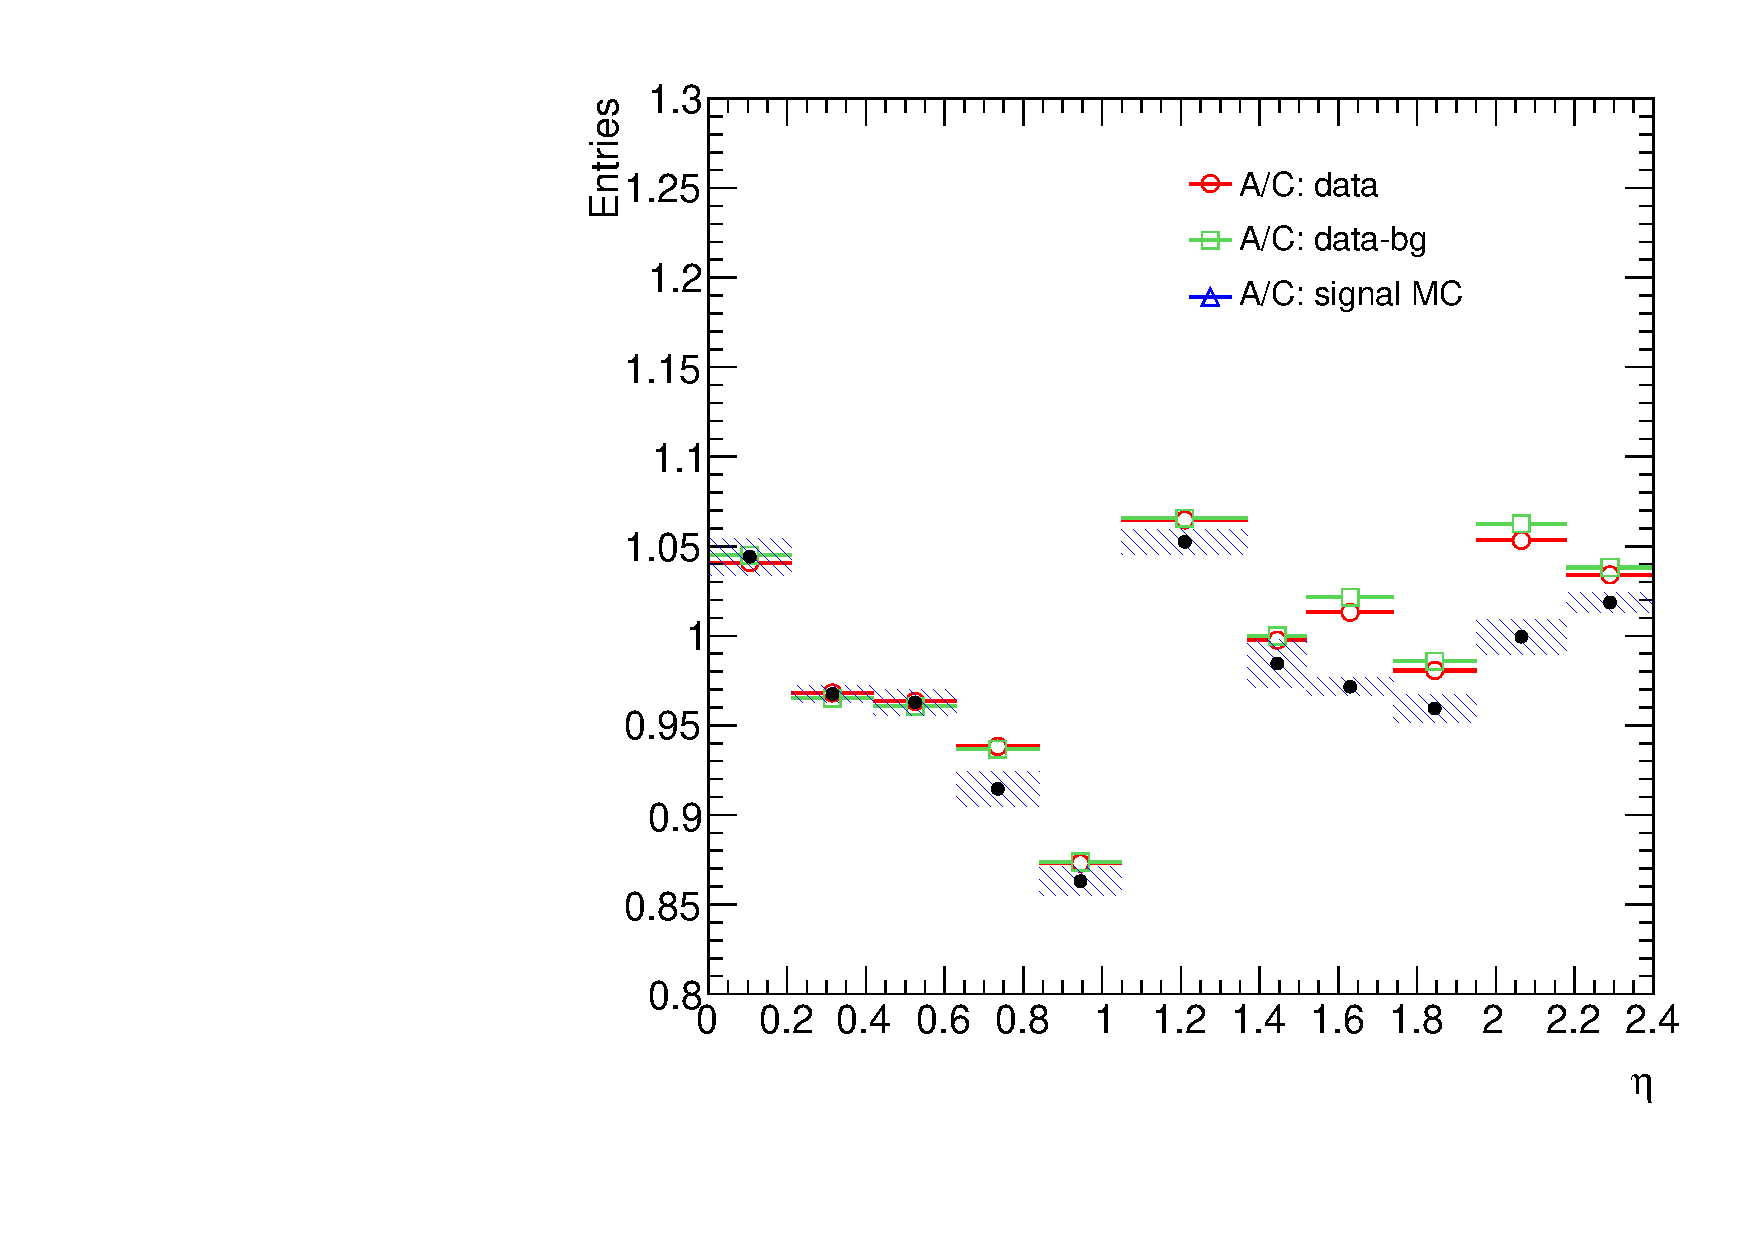
\includegraphics[width=1.0\textwidth]{dates/20130403/figures/old/ACSIDE/W_NOM_Q0_stack_d3_eta_lpt_met_y_2__1_z_0__1_POS}
\column{.5\textwidth}
\centering
\small{ $W^{-}$}
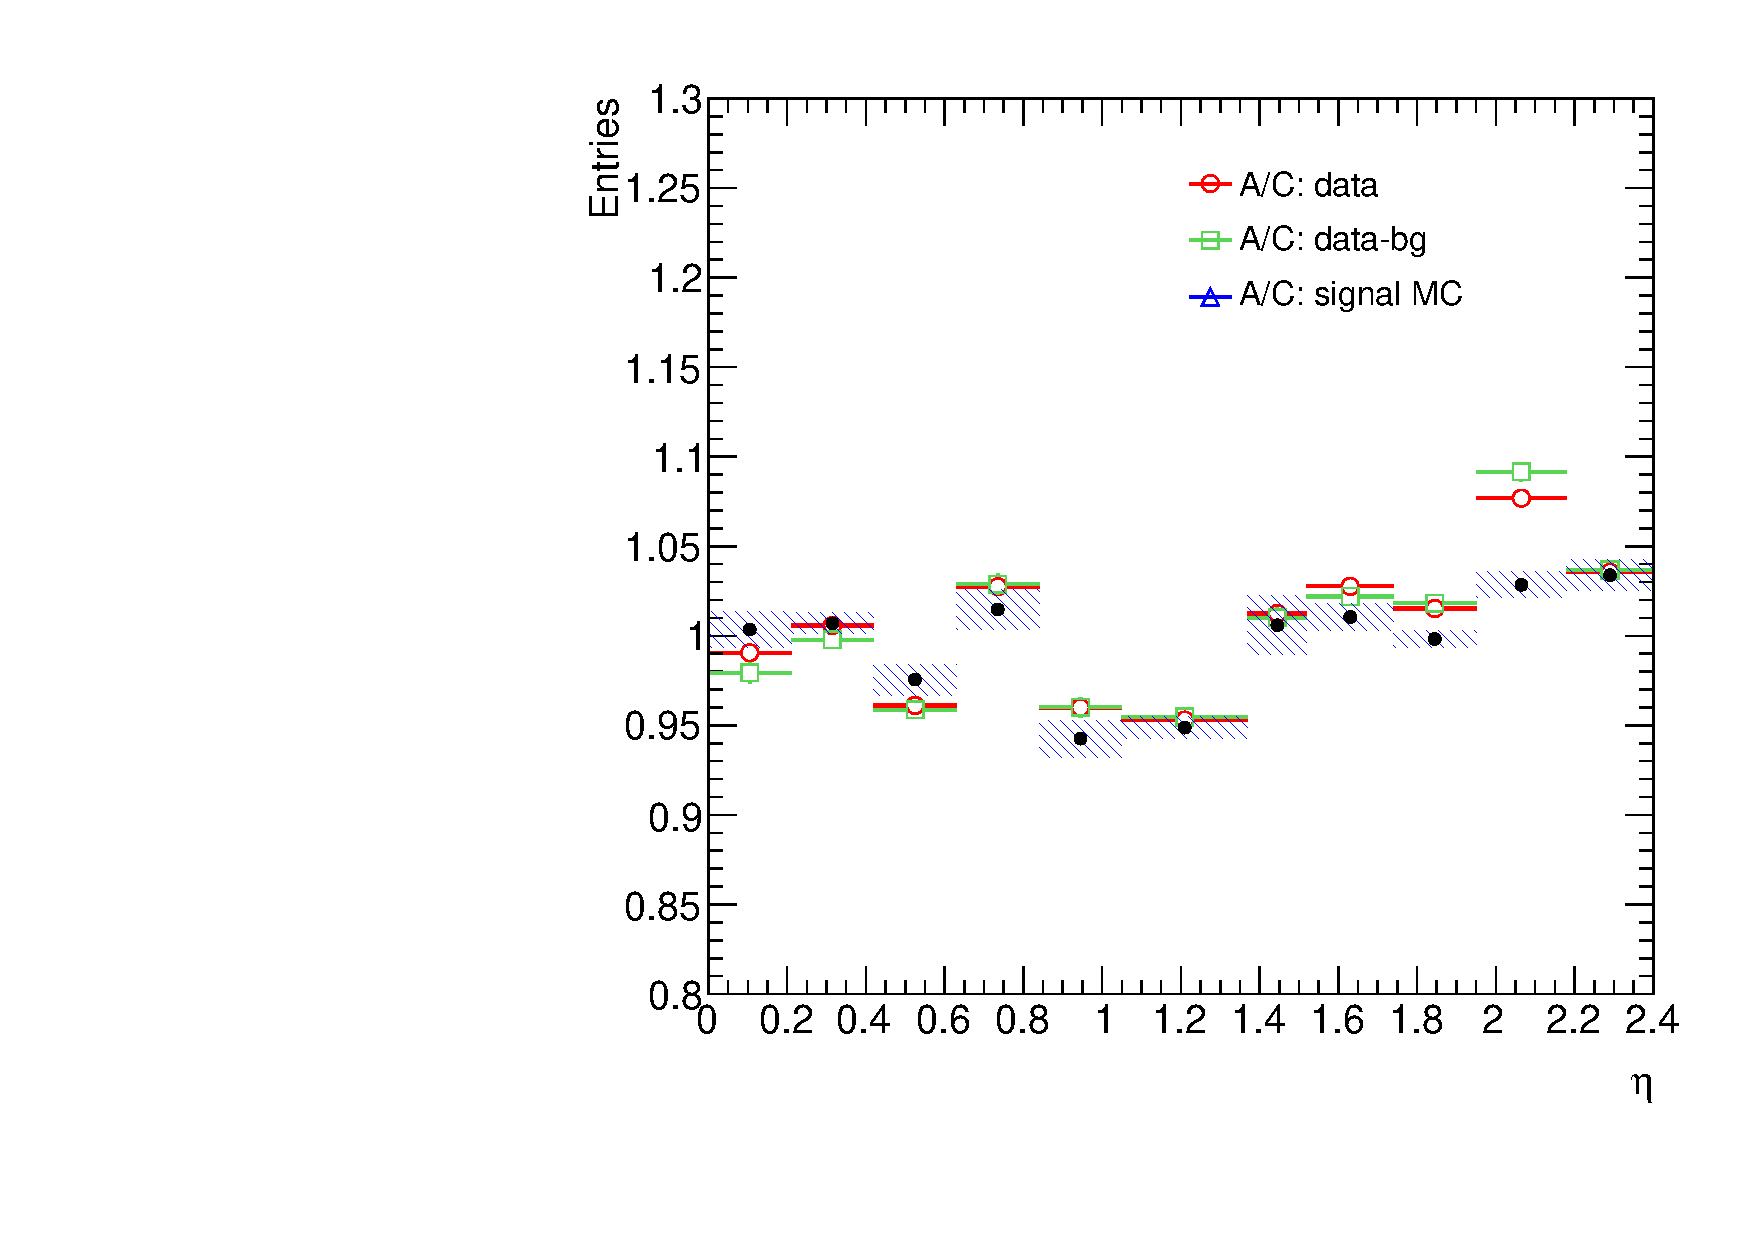
\includegraphics[width=1.0\textwidth]{dates/20130403/figures/old/ACSIDE/W_NOM_Q0_stack_d3_eta_lpt_met_y_2__1_z_0__1_NEG}
\cole
}

\slide{ LATEST: W ratio }
{
\colb[T]
\column{.5\textwidth}
\centering
\small{ $W^{+}$}
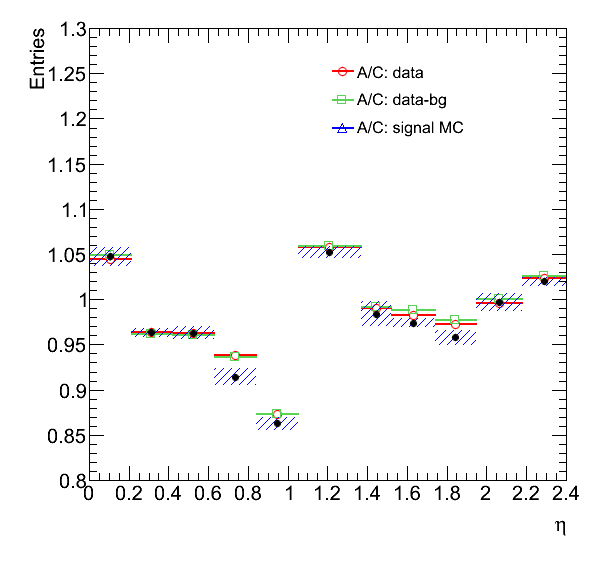
\includegraphics[width=1.0\textwidth]{dates/20130403/figures/new/ACSIDE/W_NOM_Q0_stack_d3_eta_lpt_met_y_2__1_z_0__1_POS}
\column{.5\textwidth}
\centering
\small{ $W^{-}$}
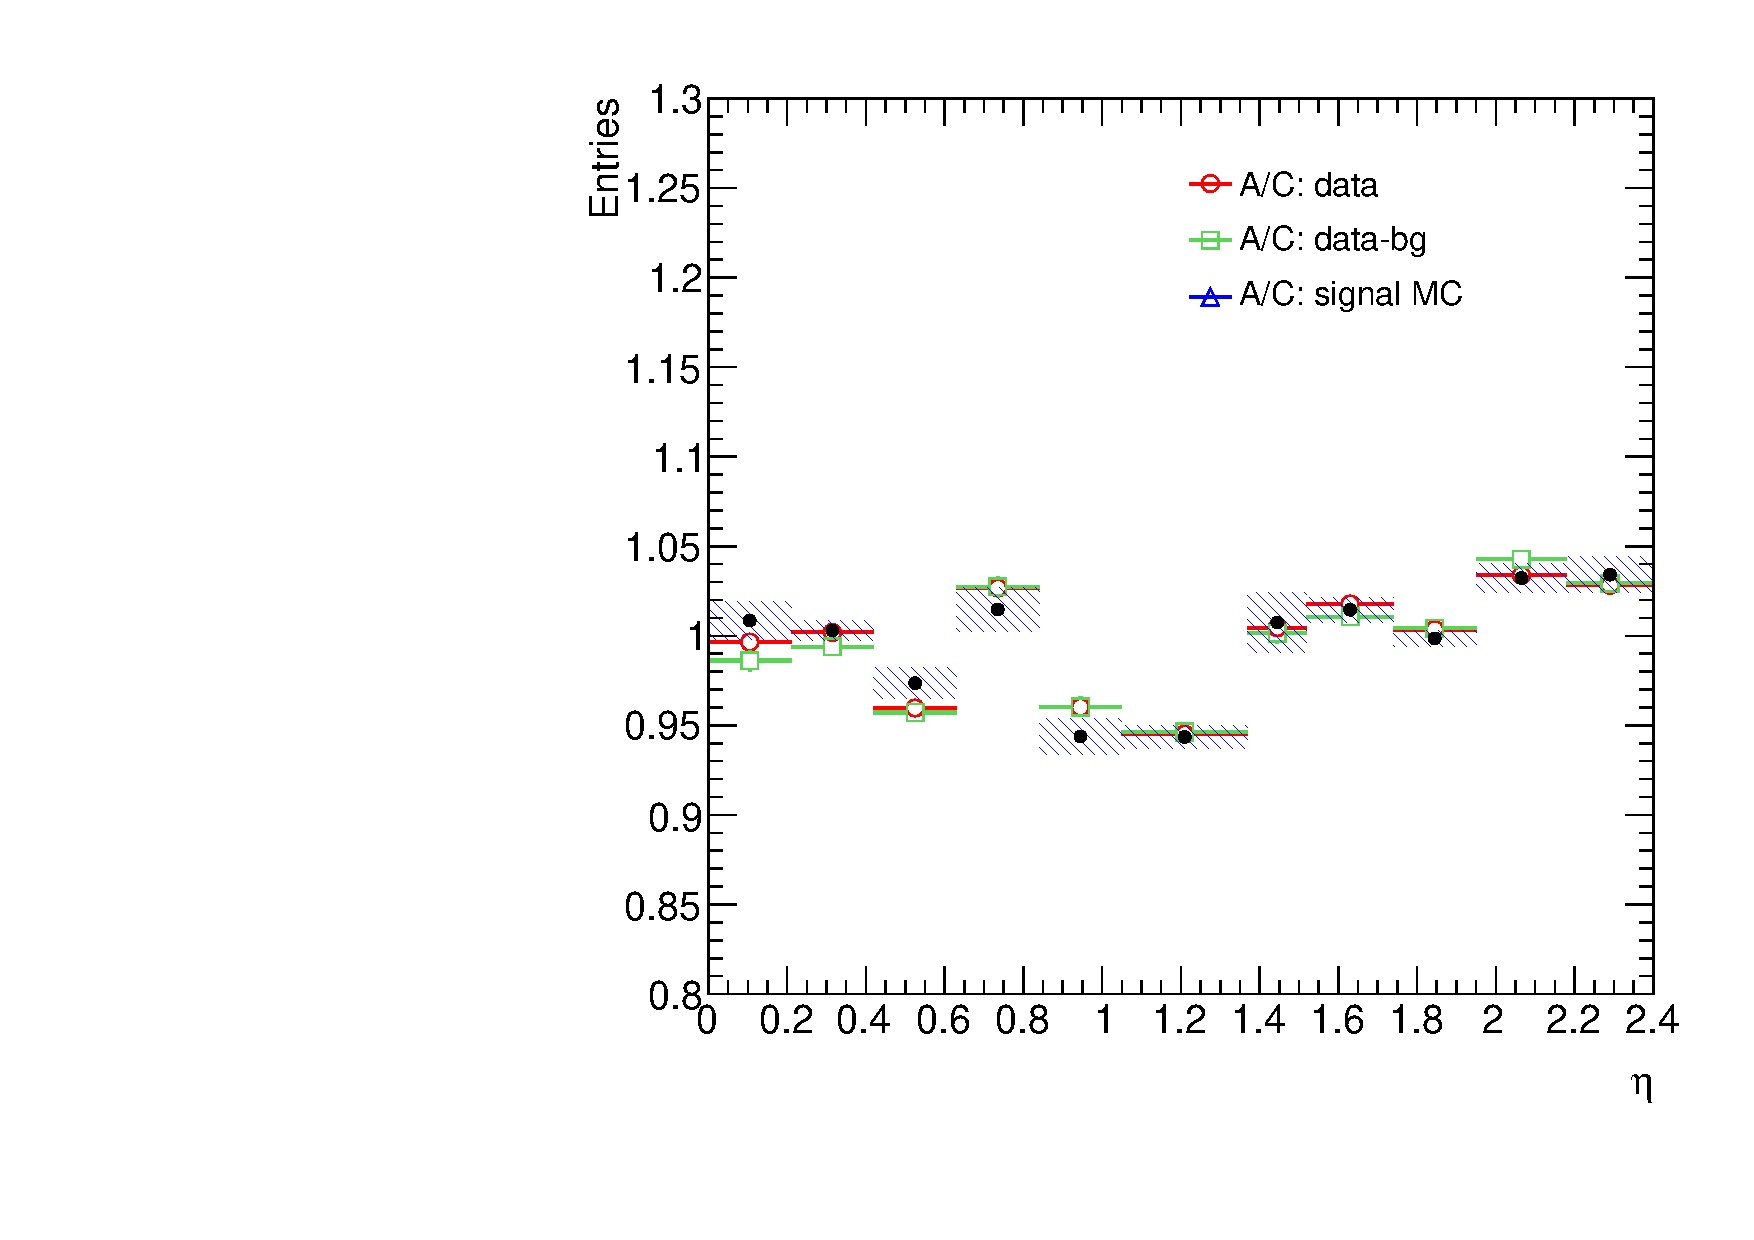
\includegraphics[width=1.0\textwidth]{dates/20130403/figures/new/ACSIDE/W_NOM_Q0_stack_d3_eta_lpt_met_y_2__1_z_0__1_NEG}
\cole
}

\slide{ mu18 vs mu18MG  } {
 Below, 2D eta-phi plots for full W selection, where:
 \iteb
 \item mu18MG trigger fails, but mu18 succeeds
 \itee
}

\slide{ mu18MG vs mu18: mu18 succeeds  } {
\colb[T]
\column{.5\textwidth}
$\mu^+$: Period D
\centering
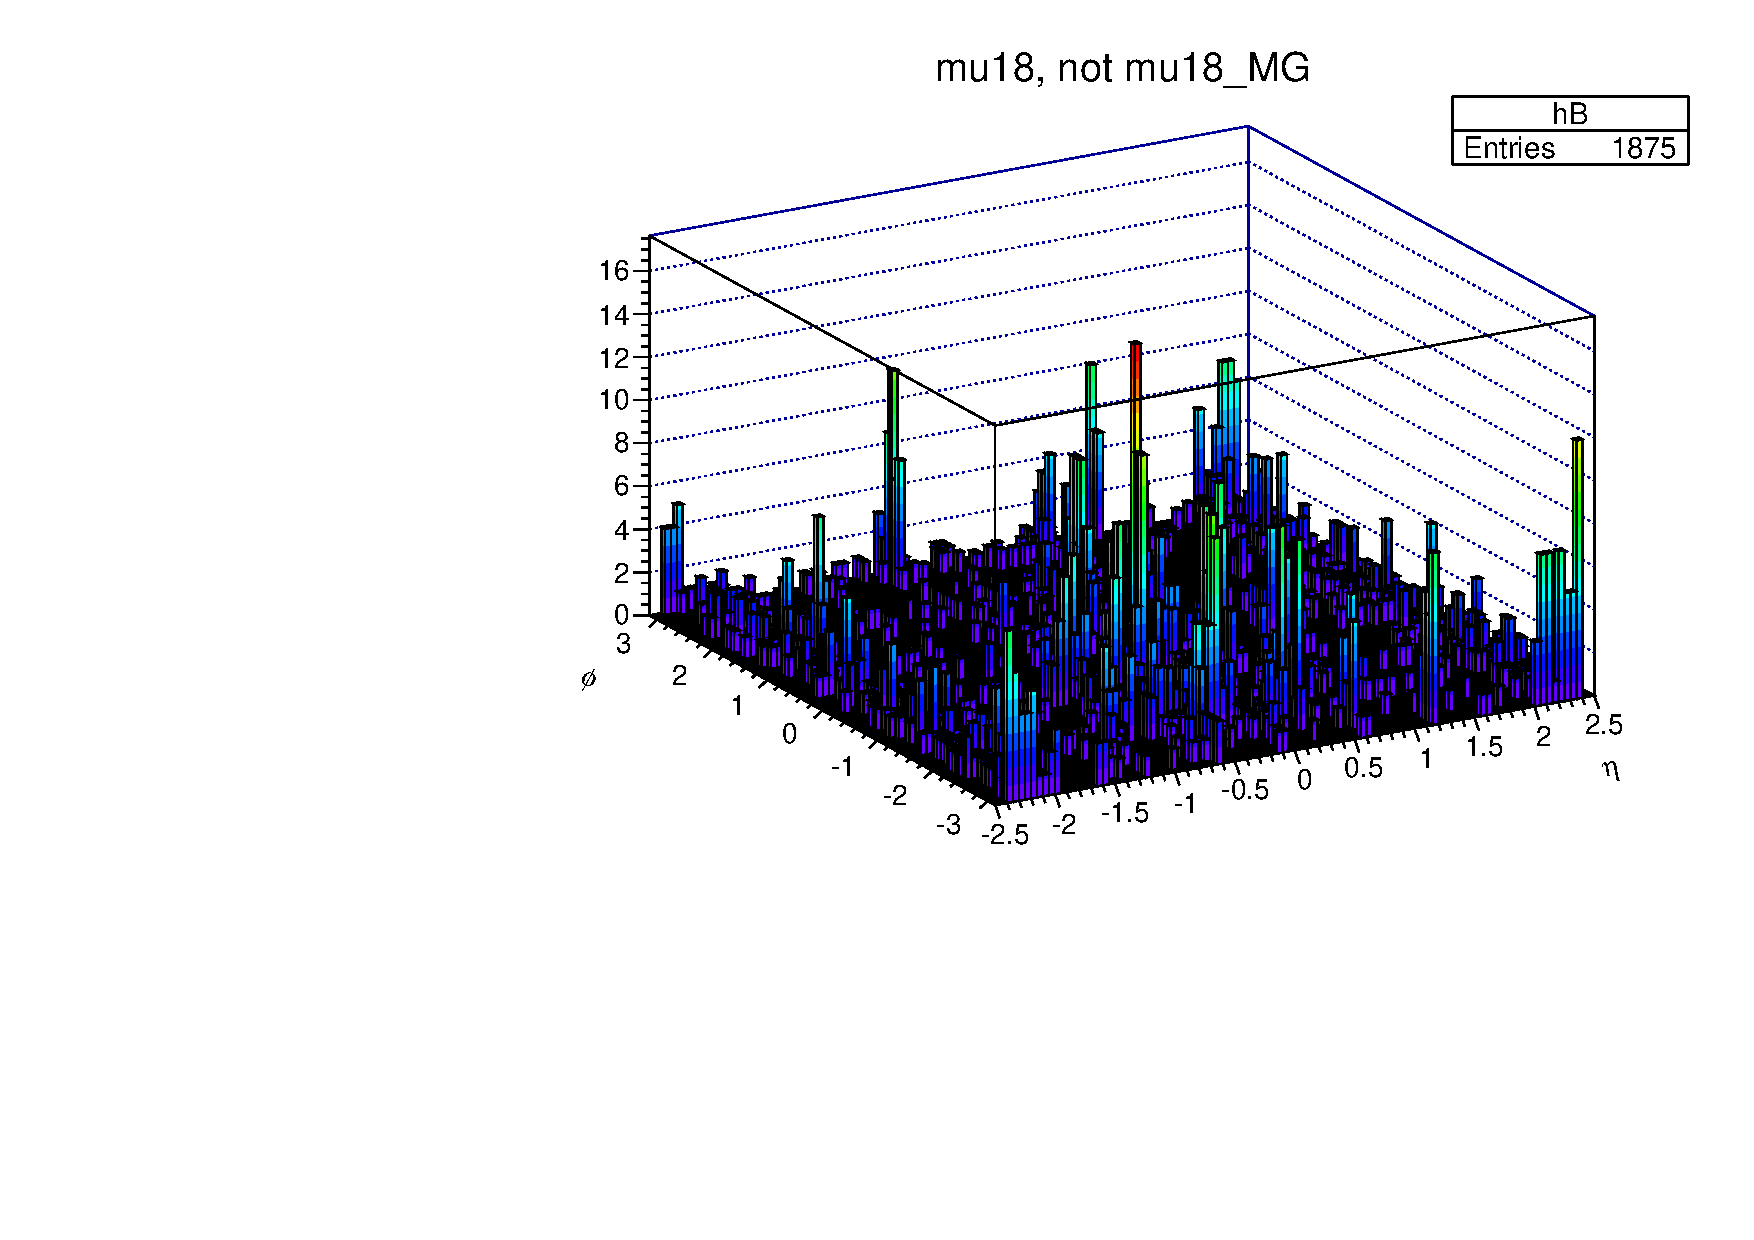
\includegraphics[width=0.95\textwidth]{dates/20130306/figures/mu18/dump_MG_dataD_w_POS.dat__MUID_NOT_MG}
\column{.5\textwidth}
$\mu^-$: Period D
\centering
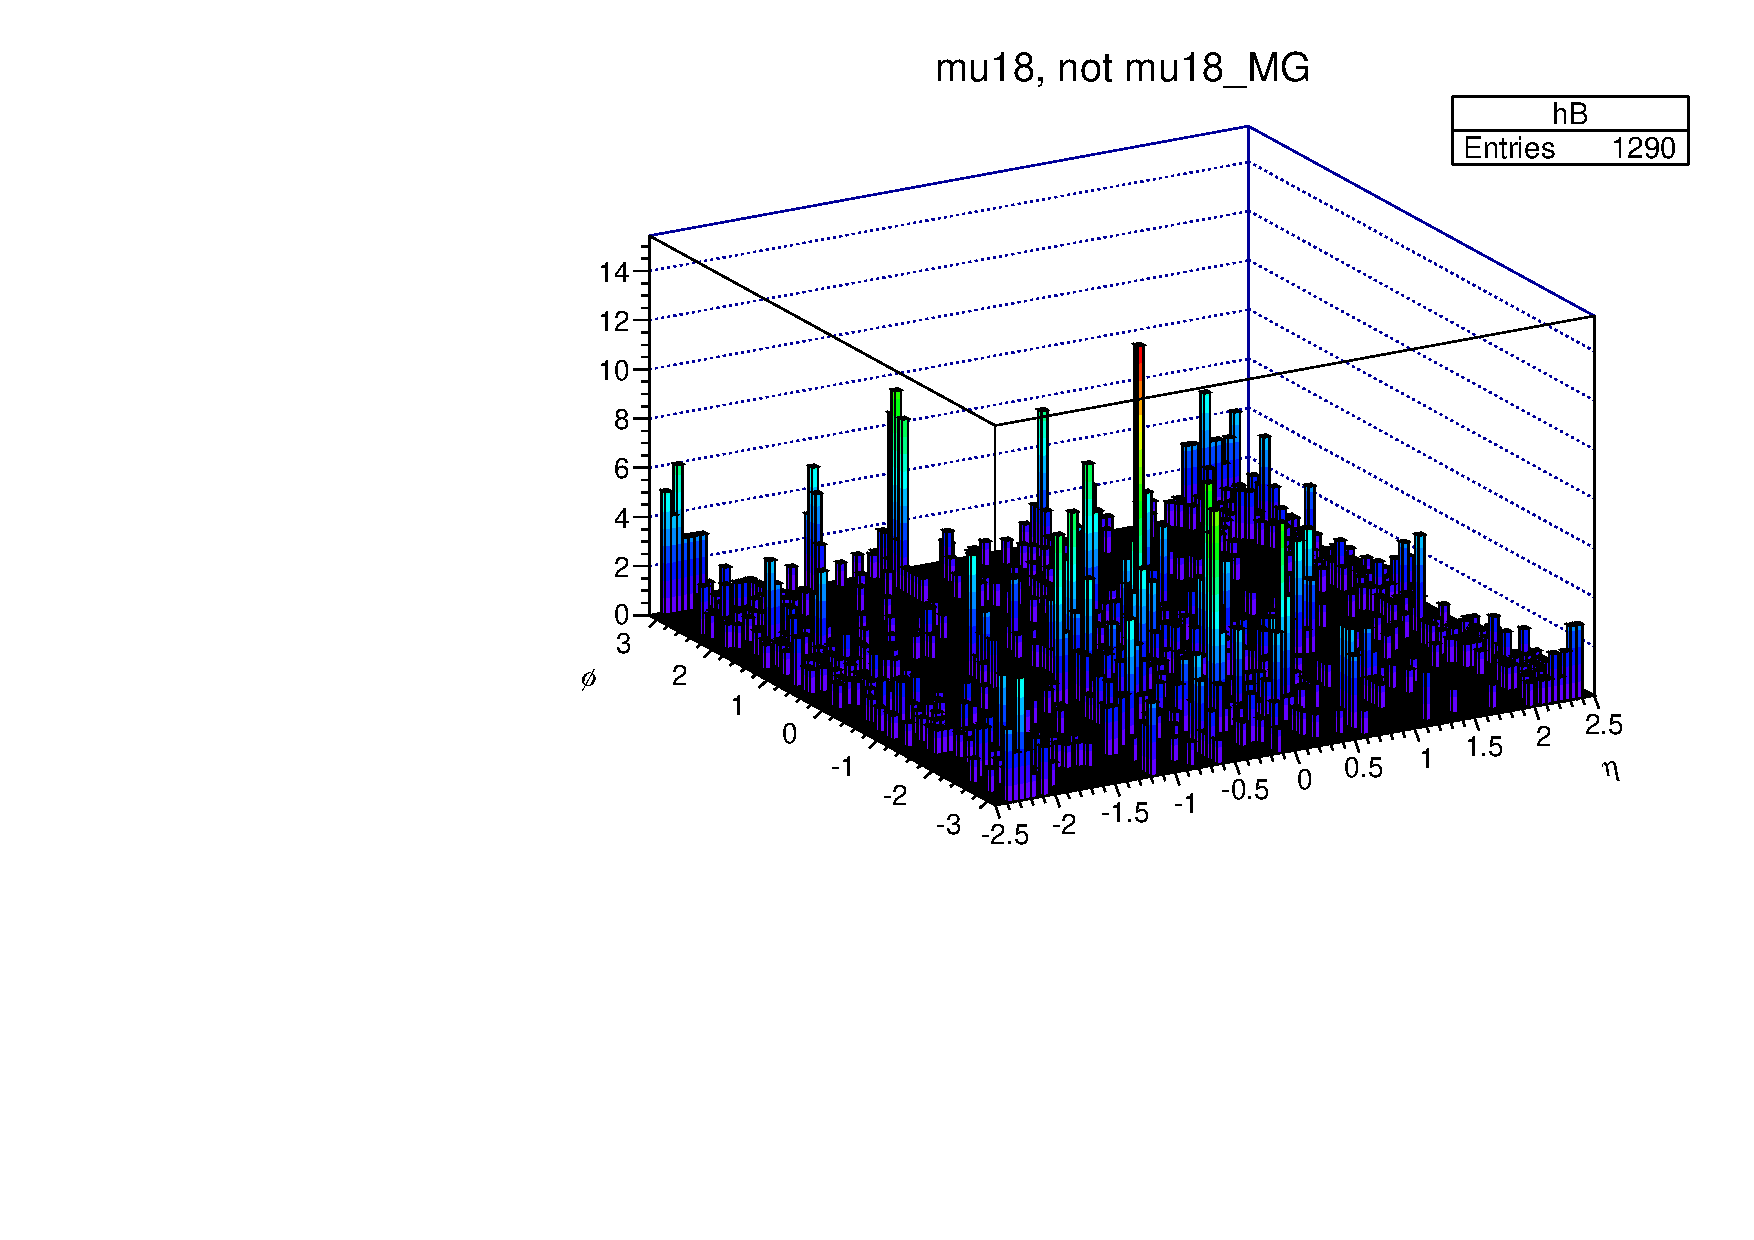
\includegraphics[width=0.95\textwidth]{dates/20130306/figures/mu18/dump_MG_dataD_w_NEG.dat__MUID_NOT_MG}
\cole
}
\slide{ mu18MG vs mu18: mu18MG succeeds  } {
\colb[T]
\column{.5\textwidth}
$\mu^+$: Period L
\centering
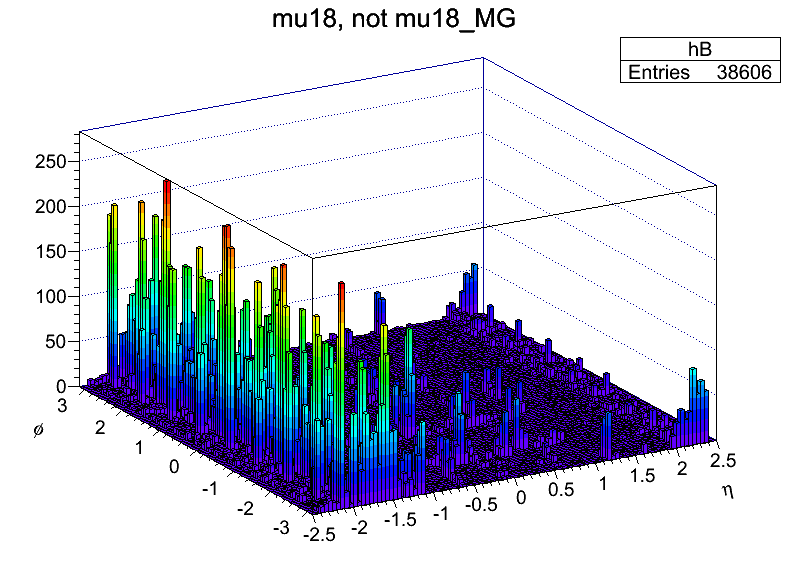
\includegraphics[width=0.95\textwidth]{dates/20130306/figures/mu18/dump_MG_dataL_w_POS.dat__MUID_NOT_MG}
\column{.5\textwidth}
$\mu^-$: Period L
\centering
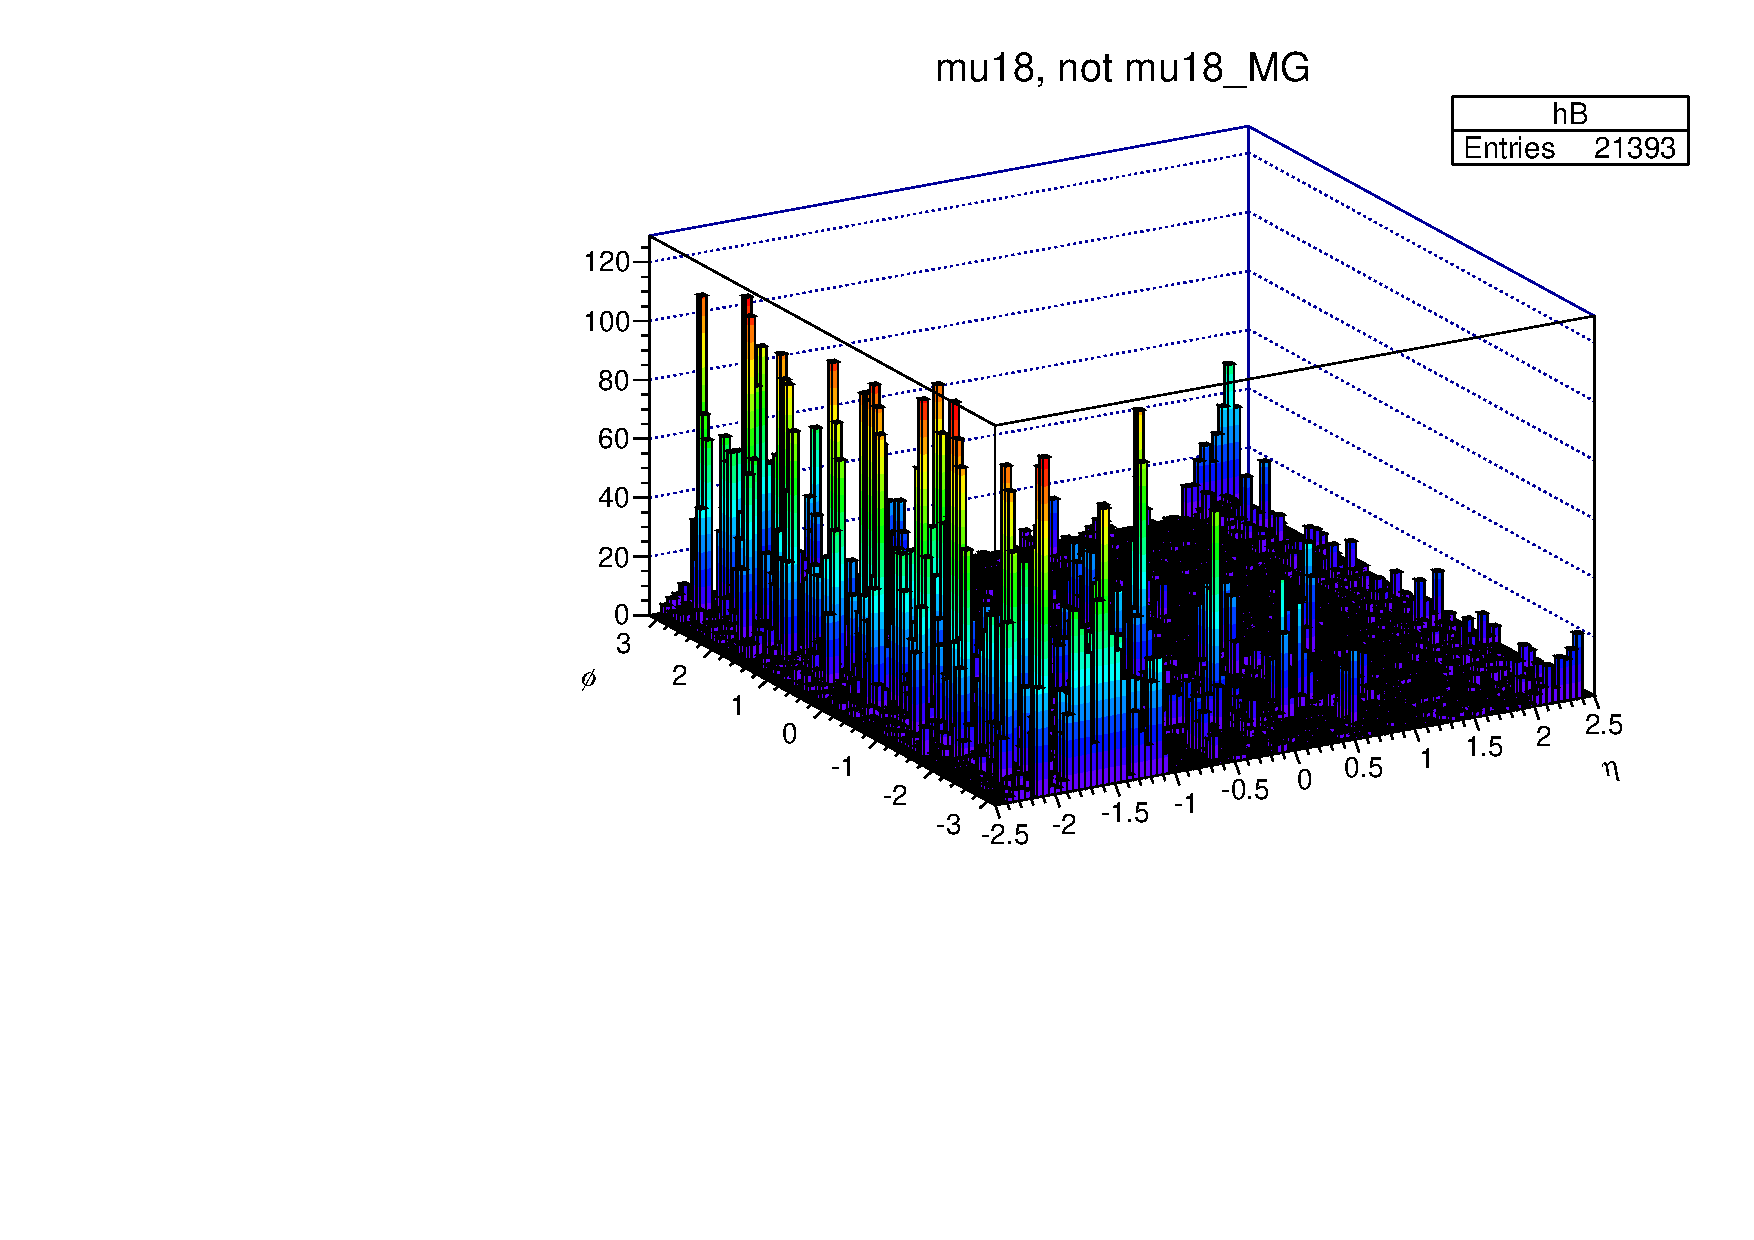
\includegraphics[width=0.95\textwidth]{dates/20130306/figures/mu18/dump_MG_dataL_w_NEG.dat__MUID_NOT_MG}
\cole
}
\slide{ mu18 vs mu18MG  } {
  Conclusions: \\
  Remember that these plots do not rely on trigger matching - we simply use W selection with 1 muon, which HAD to trigger.
  We see that \red{something happened to the MG trigger on the C-side in later data periods}. The mu18 trigger is not affected.
}

% W eta stacks
\slide{ BEFORE: W eta stacks }
{
\colb[T]
\column{.5\textwidth}
\centering
\small{ $W^{+}$}
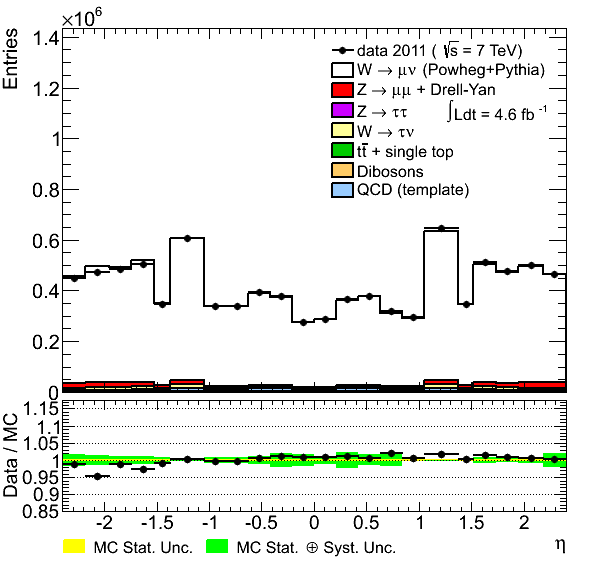
\includegraphics[width=1.0\textwidth]{dates/20130403/figures/old/STACKS/CONTROL25/P_stack_d3_eta_lpt_met_y_2__1_z_0__1_POS}
\column{.5\textwidth}
\centering
\small{ $W^{-}$}
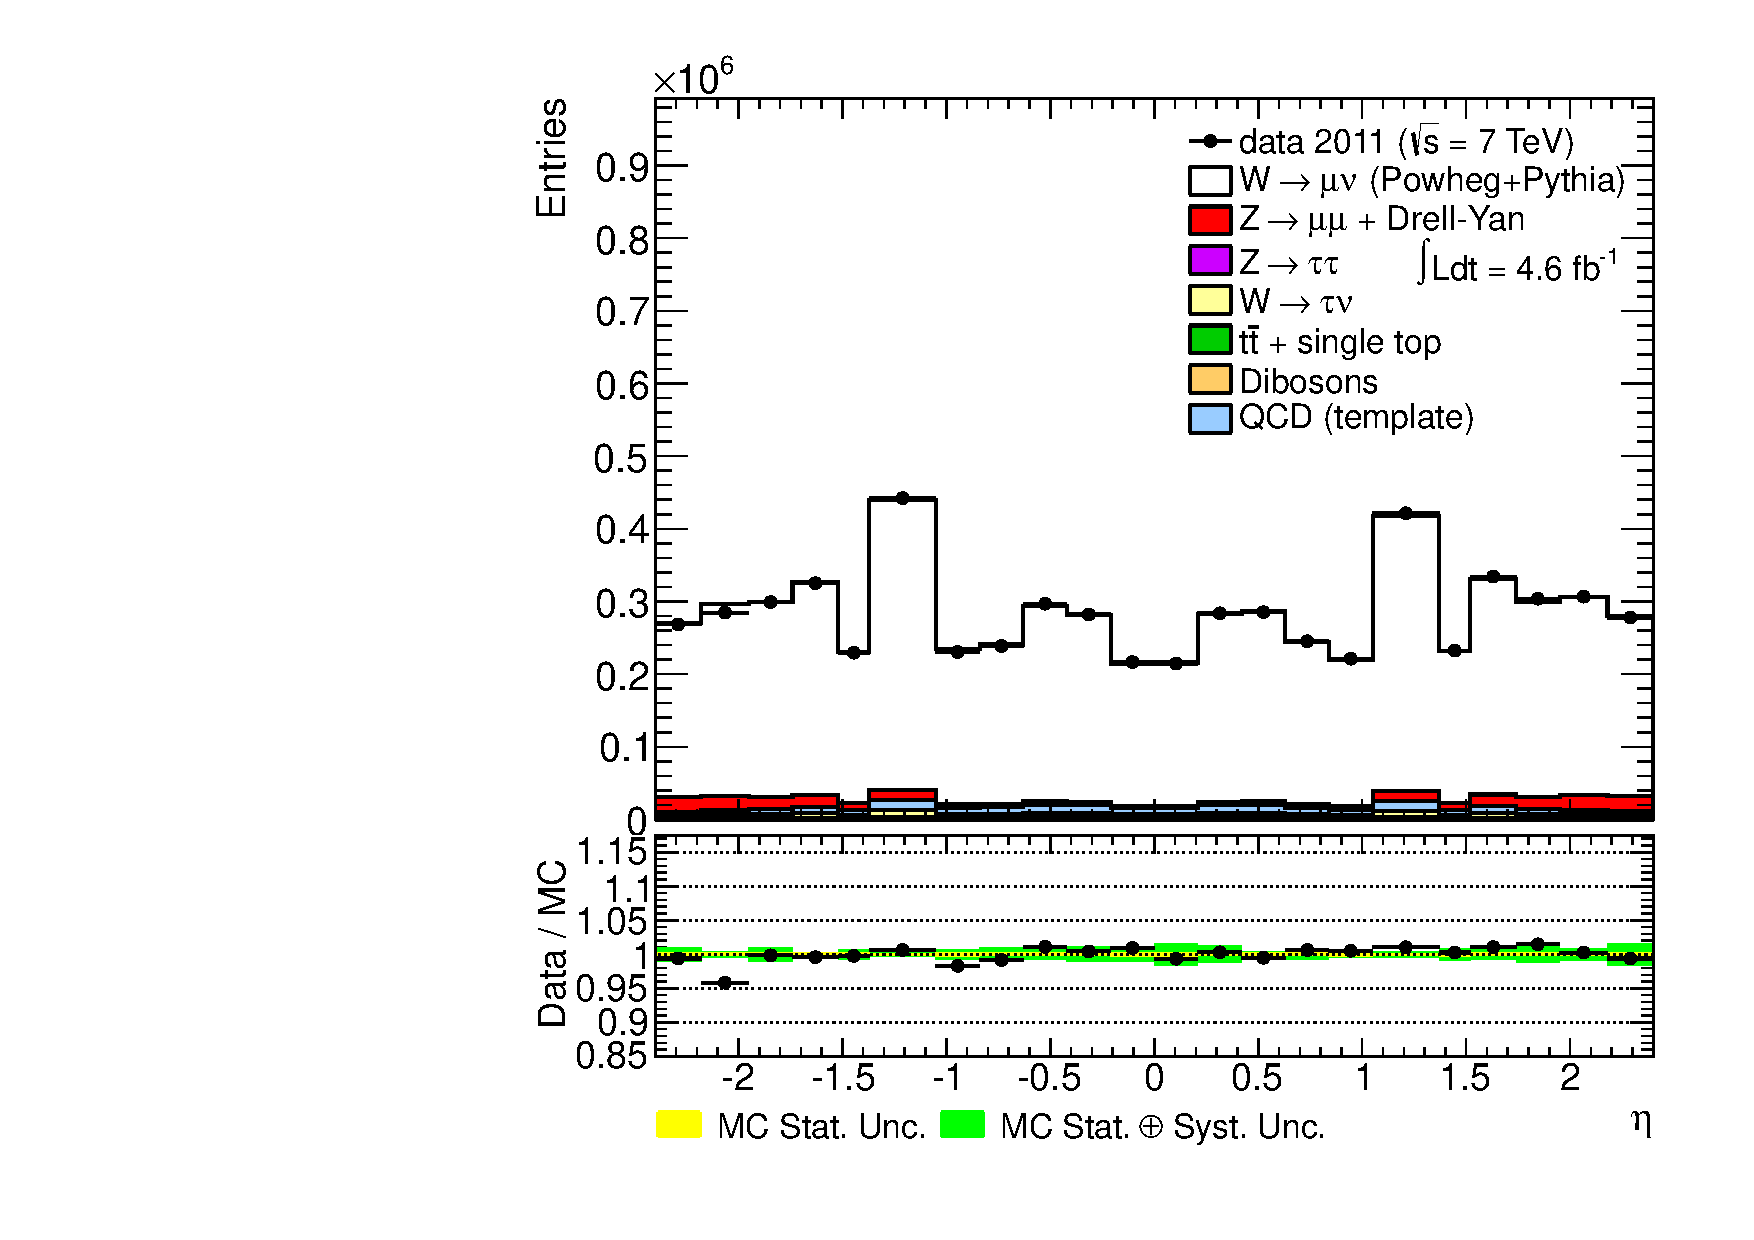
\includegraphics[width=1.0\textwidth]{dates/20130403/figures/old/STACKS/CONTROL25/P_stack_d3_eta_lpt_met_y_2__1_z_0__1_NEG}
\cole
}

\slide{ LATEST: W eta stacks }
{
\colb[T]
\column{.5\textwidth}
\centering
\small{ $W^{+}$}
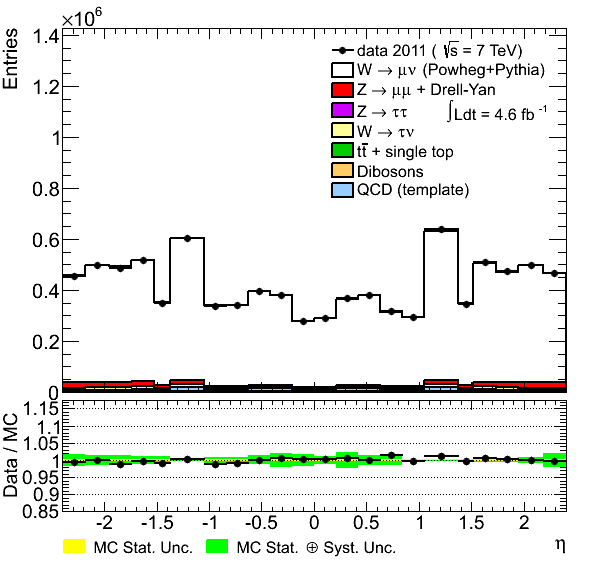
\includegraphics[width=1.0\textwidth]{dates/20130403/figures/new/STACKS/CONTROL25/P_stack_d3_eta_lpt_met_y_2__1_z_0__1_POS}
\column{.5\textwidth}
\centering
\small{ $W^{-}$}
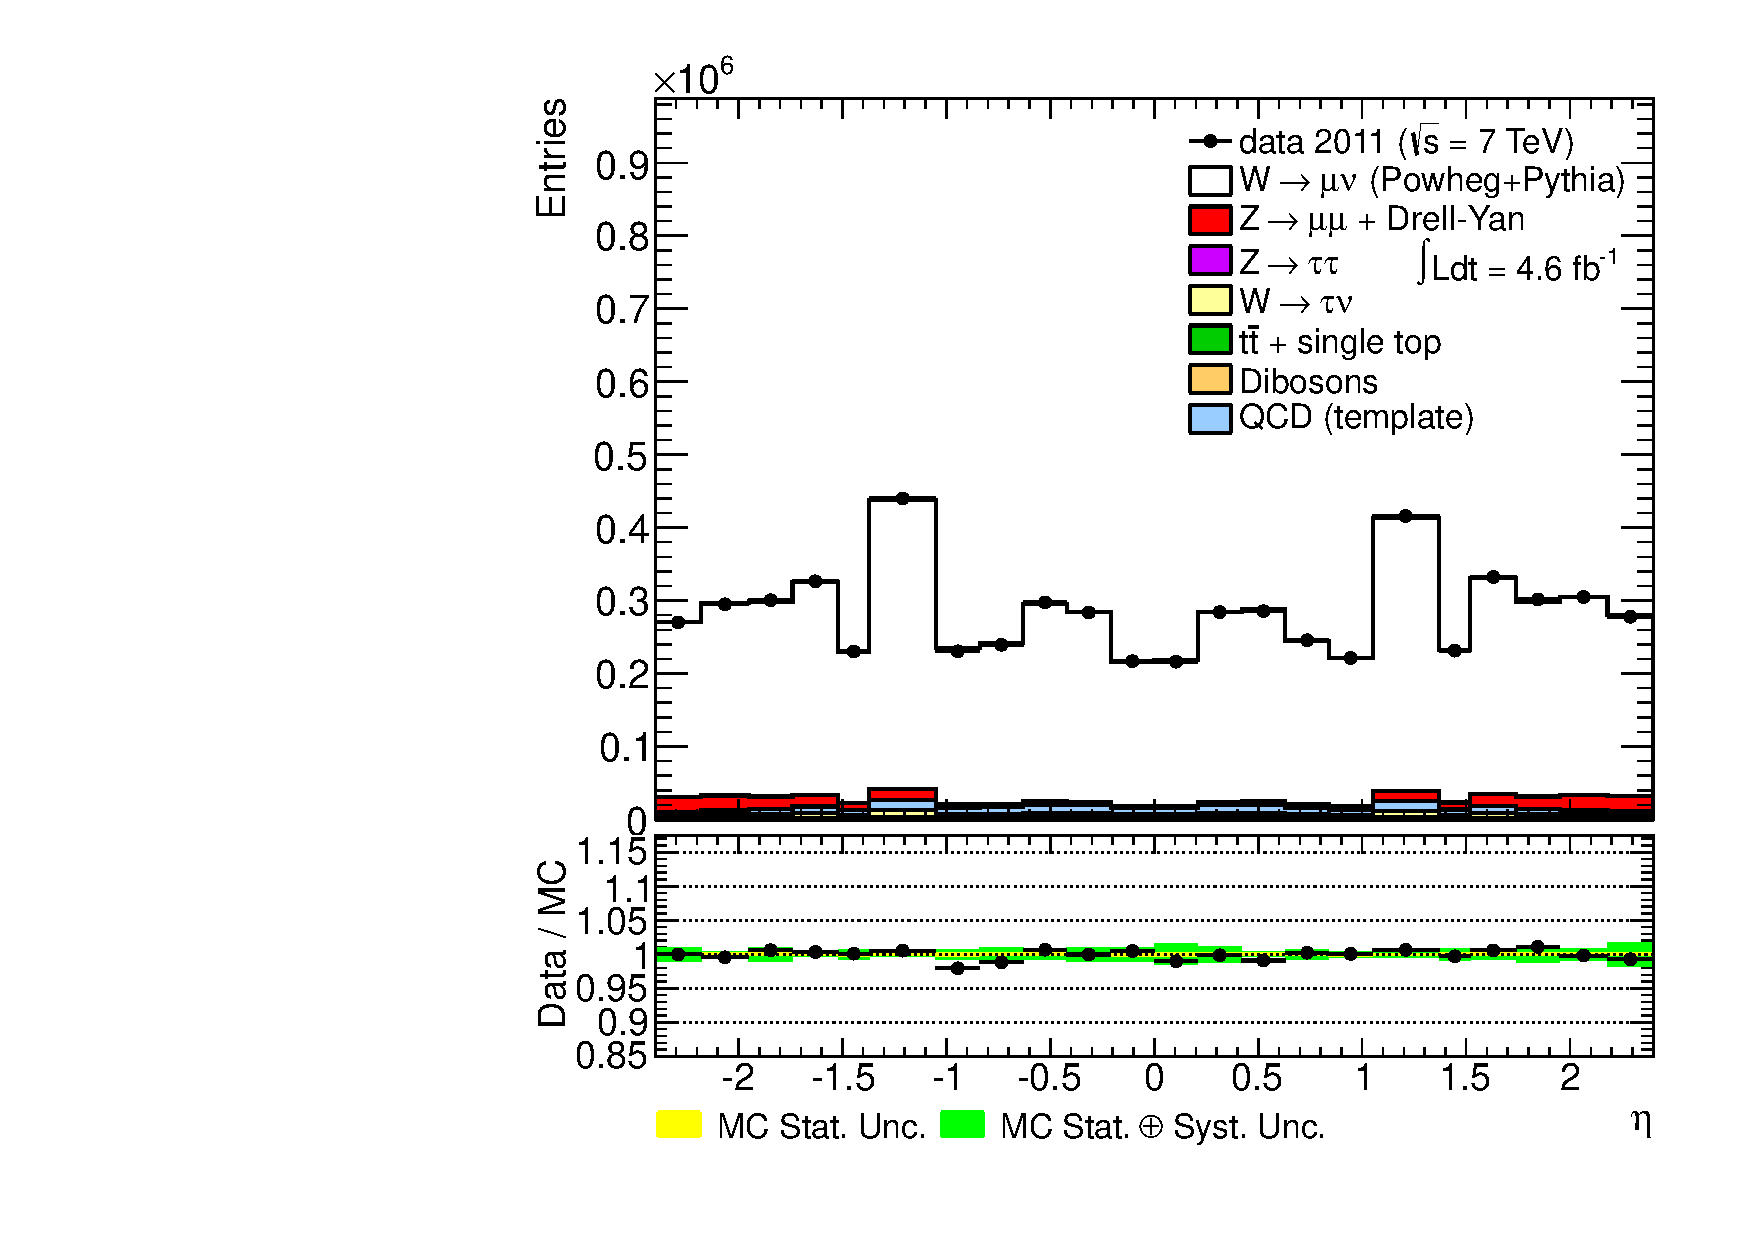
\includegraphics[width=1.0\textwidth]{dates/20130403/figures/new/STACKS/CONTROL25/P_stack_d3_eta_lpt_met_y_2__1_z_0__1_NEG}
\cole
}

% tables W-
\slide{ BEFORE: $W^-$ cross-section tables }
{
\small{
\begin{table}[tbph]
\centering
\begin{tabular}{lccccc}
\hline
\hline
$\eta$ bin & $XSEC_{|\eta|}^{ele}$ & $XSEC_{|\eta|}^{\mu}$ & $\delta$ & $XSEC_{Aside} - XSEC_{Cside}$ & $(A-C)/\delta$ \\
\hline
$0.00 < |\eta| <0.21$ & 433.0 & 432.6 & 4.1 & -9.4 & -2.3 \\
$0.21 < |\eta| <0.42$ & 428.9 & 431.3 & 4.2 & -2.2 & -0.5 \\
$0.42 < |\eta| <0.63$ & 423.8 & 425.6 & 4.7 & -7.0 & -1.5 \\
$0.63 < |\eta| <0.84$ & 418.8 & 419.7 & 3.8 & 6.8 & 1.8 \\
$0.84 < |\eta| <1.05$ & 412.0 & 408.7 & 5.1 & 11.3 & 2.2 \\
$1.05 < |\eta| <1.37$ & 406.2 & 399.9 & 5.1 & 1.4 & 0.3 \\
$1.37 < |\eta| <1.52$ & XXX.X & 382.0 & 4.5 & 1.5 & 0.3 \\
$1.52 < |\eta| <1.74$ & XXX.X & 372.9 & 4.1 & 4.9 & 1.2 \\
$1.74 < |\eta| <1.95$ & 360.4 & 358.9 & 5.2 & 4.4 & 0.9 \\
$1.95 < |\eta| <2.18$ & 339.9 & 332.4 & 3.9 & 19.5 & \color{red}{5.0} \\
$2.18 < |\eta| <2.40$ & XXX.X & 317.2 & 3.7 & -0.4 & -0.1 \\
\hline
\end{tabular}
\caption{Studying A-side vs C-side differences for $W^{-} \rightarrow \mu^{-} \nu$.}
\end{table}
}
}
\slide{ LATEST: $W^-$ cross-section tables }
{
\small{
\begin{table}[tbph]
\centering
\begin{tabular}{lccccc}
\hline
\hline
$\eta$ bin & $XSEC_{|\eta|}^{ele}$ & $XSEC_{|\eta|}^{\mu}$ & $\delta$ & $XSEC_{Aside} - XSEC_{Cside}$ & $(A-C)/\delta$ \\
\hline
$0.00 < |\eta| <0.21$ & 433.0 & 432.7 & 4.1 & -9.0 & -2.2 \\
$0.21 < |\eta| <0.42$ & 428.9 & 430.9 & 4.1 & -2.1 & -0.5 \\
$0.42 < |\eta| <0.63$ & 423.8 & 425.5 & 4.9 & -7.0 & -1.4 \\
$0.63 < |\eta| <0.84$ & 418.8 & 419.7 & 3.8 & 6.5 & 1.7 \\
$0.84 < |\eta| <1.05$ & 412.0 & 408.5 & 5.2 & 10.9 & 2.1 \\
$1.05 < |\eta| <1.37$ & 406.2 & 400.9 & 5.0 & 0.3 & 0.1 \\
$1.37 < |\eta| <1.52$ & XXX.X & 383.5 & 4.5 & -2.4 & -0.5 \\
$1.52 < |\eta| <1.74$ & XXX.X & 375.2 & 4.2 & -0.5 & -0.1 \\
$1.74 < |\eta| <1.95$ & 360.4 & 361.6 & 5.2 & -0.2 & -0.0 \\
$1.95 < |\eta| <2.18$ & 339.9 & 339.9 & 4.1 & 3.2 & 0.8 \\
$2.18 < |\eta| <2.40$ & XXX.X & 319.2 & 3.8 & -2.8 & -0.7 \\
\hline
\end{tabular}
\caption{Studying A-side vs C-side differences for $W^{-} \rightarrow \mu^{-} \nu$.}
\end{table}
}
}

% tables W+
\slide{ BEFORE: $W^+$ cross-section tables }
{
\small{
\begin{table}[tbph]
\centering
\begin{tabular}{lccccc}
\hline
\hline
$\eta$ bin & $XSEC_{|\eta|}^{ele}$ & $XSEC_{|\eta|}^{\mu}$ & $\delta$ & $XSEC_{Aside} - XSEC_{Cside}$ & $(A-C)/\delta$ \\
\hline
$0.00 < |\eta| <0.21$ & 572.5 & 572.0 & 4.7 & 1.9 & 0.4 \\
$0.21 < |\eta| <0.42$ & 571.4 & 575.4 & 4.6 & -1.9 & -0.4 \\
$0.42 < |\eta| <0.63$ & 572.5 & 574.4 & 7.0 & 0.7 & 0.1 \\
$0.63 < |\eta| <0.84$ & 579.0 & 579.5 & 4.6 & 14.2 & \color{red}{3.1} \\
$0.84 < |\eta| <1.05$ & 582.6 & 579.3 & 5.3 & 7.1 & 1.3 \\
$1.05 < |\eta| <1.37$ & 596.2 & 591.0 & 5.9 & 8.9 & 1.5 \\
$1.37 < |\eta| <1.52$ & XXX.X & 588.0 & 6.4 & 7.3 & 1.1 \\
$1.52 < |\eta| <1.74$ & XXX.X & 588.7 & 5.6 & 26.6 & \color{red}{4.7} \\
$1.74 < |\eta| <1.95$ & 596.9 & 593.0 & 4.4 & 13.4 & \color{red}{3.1} \\
$1.95 < |\eta| <2.18$ & 584.8 & 572.4 & 7.1 & 32.5 & \color{red}{4.6} \\
$2.18 < |\eta| <2.40$ & XXX.X & 560.0 & 6.4 & 10.1 & 1.6 \\
\hline
\end{tabular}
\caption{Studying A-side vs C-side differences for $W^{+} \rightarrow \mu^{+} \nu$.}
\end{table}
}
}
\slide{ LATEST: $W^+$ cross-section tables }
{
\small{
\begin{table}[tbph]
\centering
\begin{tabular}{lccccc}
\hline
\hline
$\eta$ bin & $XSEC_{|\eta|}^{ele}$ & $XSEC_{|\eta|}^{\mu}$ & $\delta$ & $XSEC_{Aside} - XSEC_{Cside}$ & $(A-C)/\delta$ \\
\hline
$0.00 < |\eta| <0.21$ & 572.5 & 572.2 & 4.7 & 2.5 & 0.5 \\
$0.21 < |\eta| <0.42$ & 571.4 & 575.3 & 4.7 & -1.8 & -0.4 \\
$0.42 < |\eta| <0.63$ & 572.5 & 574.9 & 6.9 & 0.3 & 0.0 \\
$0.63 < |\eta| <0.84$ & 579.0 & 579.8 & 4.6 & 14.4 & \color{red}{3.1} \\
$0.84 < |\eta| <1.05$ & 582.6 & 578.8 & 5.2 & 7.4 & 1.4 \\
$1.05 < |\eta| <1.37$ & 596.2 & 593.0 & 5.7 & 5.2 & 0.9 \\
$1.37 < |\eta| <1.52$ & XXX.X & 590.5 & 6.4 & 3.0 & 0.5 \\
$1.52 < |\eta| <1.74$ & XXX.X & 598.8 & 6.0 & 6.2 & 1.0 \\
$1.74 < |\eta| <1.95$ & 596.9 & 595.7 & 4.4 & 9.5 & 2.1 \\
$1.95 < |\eta| <2.18$ & 584.8 & 590.1 & 7.2 & 0.0 & 0.0 \\
$2.18 < |\eta| <2.40$ & XXX.X & 564.1 & 7.0 & 3.1 & 0.4 \\
\hline
\end{tabular}
\caption{Studying A-side vs C-side differences for $W^{+} \rightarrow \mu^{+} \nu$.}
\end{table}
}
}

%%%%%%% Back-up slides %%%%%%%%%%
\appendix
\newcounter{finalframe}
\setcounter{finalframe}{\value{framenumber}}

\slide{}
{

\centering
\Huge Back-up slides
}
